\documentclass[a4paper, 11pt]{article}
\usepackage[utf8]{inputenc}
\usepackage{amssymb,amsmath,amsthm}
\usepackage{geometry}
\usepackage[T1]{fontenc}
\usepackage[french]{babel}
\usepackage{fontawesome}
\usepackage{pifont}
\usepackage{tcolorbox}
\usepackage{fancybox}
\usepackage{bbold}
\usepackage{tkz-tab}
\usepackage{tikz}
\usepackage{fancyhdr}
\usepackage{sectsty}
\usepackage[framemethod=TikZ]{mdframed}
\usepackage{stackengine}
\usepackage{scalerel}
\usepackage{xcolor}
\usepackage{hyperref}
\usepackage{listings}
\usepackage{enumitem}
\usepackage{stmaryrd} 
\usepackage{comment}


\hypersetup{
    colorlinks=true,
    urlcolor=blue,
    linkcolor=blue,
    breaklinks=true
}





\theoremstyle{definition}
\newtheorem{probleme}{Problème}
\theoremstyle{definition}


%%%%% box environement 
\newenvironment{fminipage}%
     {\begin{Sbox}\begin{minipage}}%
     {\end{minipage}\end{Sbox}\fbox{\TheSbox}}

\newenvironment{dboxminipage}%
     {\begin{Sbox}\begin{minipage}}%
     {\end{minipage}\end{Sbox}\doublebox{\TheSbox}}


%\fancyhead[R]{Chapitre 1 : Nombres}


\newenvironment{remarques}{ 
\paragraph{Remarques :}
	\begin{list}{$\bullet$}{}
}{
	\end{list}
}




\newtcolorbox{tcbdoublebox}[1][]{%
  sharp corners,
  colback=white,
  fontupper={\setlength{\parindent}{20pt}},
  #1
}







%Section
% \pretocmd{\section}{%
%   \ifnum\value{section}=0 \else\clearpage\fi
% }{}{}



\sectionfont{\normalfont\Large \bfseries \underline }
\subsectionfont{\normalfont\Large\itshape\underline}
\subsubsectionfont{\normalfont\large\itshape\underline}



%% Format théoreme, defintion, proposition.. 
\newmdtheoremenv[roundcorner = 5px,
leftmargin=15px,
rightmargin=30px,
innertopmargin=0px,
nobreak=true
]{theorem}{Théorème}

\newmdtheoremenv[roundcorner = 5px,
leftmargin=15px,
rightmargin=30px,
innertopmargin=0px,
]{theorem_break}[theorem]{Théorème}

\newmdtheoremenv[roundcorner = 5px,
leftmargin=15px,
rightmargin=30px,
innertopmargin=0px,
nobreak=true
]{corollaire}[theorem]{Corollaire}
\newcounter{defiCounter}
\usepackage{mdframed}
\newmdtheoremenv[%
roundcorner=5px,
innertopmargin=0px,
leftmargin=15px,
rightmargin=30px,
nobreak=true
]{defi}[defiCounter]{Définition}

\newmdtheoremenv[roundcorner = 5px,
leftmargin=15px,
rightmargin=30px,
innertopmargin=0px,
nobreak=true
]{prop}[theorem]{Proposition}

\newmdtheoremenv[roundcorner = 5px,
leftmargin=15px,
rightmargin=30px,
innertopmargin=0px,
]{prop_break}[theorem]{Proposition}

\newmdtheoremenv[roundcorner = 5px,
leftmargin=15px,
rightmargin=30px,
innertopmargin=0px,
nobreak=true
]{regles}[theorem]{Règles de calculs}


\newtheorem*{exemples}{Exemples}
\newtheorem{exemple}{Exemple}
\newtheorem*{rem}{Remarque}
\newtheorem*{rems}{Remarques}
% Warning sign

\newcommand\warning[1][4ex]{%
  \renewcommand\stacktype{L}%
  \scaleto{\stackon[1.3pt]{\color{red}$\triangle$}{\tiny\bfseries !}}{#1}%
}


\newtheorem{exo}{Exercice}
\newcounter{ExoCounter}
\newtheorem{exercice}[ExoCounter]{Exercice}

\newcounter{counterCorrection}
\newtheorem{correction}[counterCorrection]{\color{red}{Correction}}


\theoremstyle{definition}

%\newtheorem{prop}[theorem]{Proposition}
%\newtheorem{\defi}[1]{
%\begin{tcolorbox}[width=14cm]
%#1
%\end{tcolorbox}
%}


%--------------------------------------- 
% Document
%--------------------------------------- 






\lstset{numbers=left, numberstyle=\tiny, stepnumber=1, numbersep=5pt}




% Header et footer

\pagestyle{fancy}
\fancyhead{}
\fancyfoot{}
\renewcommand{\headwidth}{\textwidth}
\renewcommand{\footrulewidth}{0.4pt}
\renewcommand{\headrulewidth}{0pt}
\renewcommand{\footruleskip}{5px}

\fancyfoot[R]{Olivier Glorieux}
%\fancyfoot[R]{Jules Glorieux}

\fancyfoot[C]{ Page \thepage }
\fancyfoot[L]{1BIOA - Lycée Chaptal}
%\fancyfoot[L]{MP*-Lycée Chaptal}
%\fancyfoot[L]{Famille Lapin}



\newcommand{\Hyp}{\mathbb{H}}
\newcommand{\C}{\mathcal{C}}
\newcommand{\U}{\mathcal{U}}
\newcommand{\R}{\mathbb{R}}
\newcommand{\T}{\mathbb{T}}
\newcommand{\D}{\mathbb{D}}
\newcommand{\N}{\mathbb{N}}
\newcommand{\Z}{\mathbb{Z}}
\newcommand{\F}{\mathcal{F}}




\newcommand{\bA}{\mathbb{A}}
\newcommand{\bB}{\mathbb{B}}
\newcommand{\bC}{\mathbb{C}}
\newcommand{\bD}{\mathbb{D}}
\newcommand{\bE}{\mathbb{E}}
\newcommand{\bF}{\mathbb{F}}
\newcommand{\bG}{\mathbb{G}}
\newcommand{\bH}{\mathbb{H}}
\newcommand{\bI}{\mathbb{I}}
\newcommand{\bJ}{\mathbb{J}}
\newcommand{\bK}{\mathbb{K}}
\newcommand{\bL}{\mathbb{L}}
\newcommand{\bM}{\mathbb{M}}
\newcommand{\bN}{\mathbb{N}}
\newcommand{\bO}{\mathbb{O}}
\newcommand{\bP}{\mathbb{P}}
\newcommand{\bQ}{\mathbb{Q}}
\newcommand{\bR}{\mathbb{R}}
\newcommand{\bS}{\mathbb{S}}
\newcommand{\bT}{\mathbb{T}}
\newcommand{\bU}{\mathbb{U}}
\newcommand{\bV}{\mathbb{V}}
\newcommand{\bW}{\mathbb{W}}
\newcommand{\bX}{\mathbb{X}}
\newcommand{\bY}{\mathbb{Y}}
\newcommand{\bZ}{\mathbb{Z}}



\newcommand{\cA}{\mathcal{A}}
\newcommand{\cB}{\mathcal{B}}
\newcommand{\cC}{\mathcal{C}}
\newcommand{\cD}{\mathcal{D}}
\newcommand{\cE}{\mathcal{E}}
\newcommand{\cF}{\mathcal{F}}
\newcommand{\cG}{\mathcal{G}}
\newcommand{\cH}{\mathcal{H}}
\newcommand{\cI}{\mathcal{I}}
\newcommand{\cJ}{\mathcal{J}}
\newcommand{\cK}{\mathcal{K}}
\newcommand{\cL}{\mathcal{L}}
\newcommand{\cM}{\mathcal{M}}
\newcommand{\cN}{\mathcal{N}}
\newcommand{\cO}{\mathcal{O}}
\newcommand{\cP}{\mathcal{P}}
\newcommand{\cQ}{\mathcal{Q}}
\newcommand{\cR}{\mathcal{R}}
\newcommand{\cS}{\mathcal{S}}
\newcommand{\cT}{\mathcal{T}}
\newcommand{\cU}{\mathcal{U}}
\newcommand{\cV}{\mathcal{V}}
\newcommand{\cW}{\mathcal{W}}
\newcommand{\cX}{\mathcal{X}}
\newcommand{\cY}{\mathcal{Y}}
\newcommand{\cZ}{\mathcal{Z}}







\renewcommand{\phi}{\varphi}
\newcommand{\ddp}{\displaystyle}


\newcommand{\G}{\Gamma}
\newcommand{\g}{\gamma}

\newcommand{\tv}{\rightarrow}
\newcommand{\wt}{\widetilde}
\newcommand{\ssi}{\Leftrightarrow}

\newcommand{\floor}[1]{\left \lfloor #1\right \rfloor}
\newcommand{\rg}{ \mathrm{rg}}
\newcommand{\quadou}{ \quad \text{ ou } \quad}
\newcommand{\quadet}{ \quad \text{ et } \quad}
\newcommand\fillin[1][3cm]{\makebox[#1]{\dotfill}}
\newcommand\cadre[1]{[#1]}
\newcommand{\vsec}{\vspace{0.3cm}}

\DeclareMathOperator{\im}{Im}
\DeclareMathOperator{\cov}{Cov}
\DeclareMathOperator{\vect}{Vect}
\DeclareMathOperator{\Vect}{Vect}
\DeclareMathOperator{\card}{Card}
\DeclareMathOperator{\Card}{Card}
\DeclareMathOperator{\Id}{Id}
\DeclareMathOperator{\PSL}{PSL}
\DeclareMathOperator{\PGL}{PGL}
\DeclareMathOperator{\SL}{SL}
\DeclareMathOperator{\GL}{GL}
\DeclareMathOperator{\SO}{SO}
\DeclareMathOperator{\SU}{SU}
\DeclareMathOperator{\Sp}{Sp}


\DeclareMathOperator{\sh}{sh}
\DeclareMathOperator{\ch}{ch}
\DeclareMathOperator{\argch}{argch}
\DeclareMathOperator{\argsh}{argsh}
\DeclareMathOperator{\imag}{Im}
\DeclareMathOperator{\reel}{Re}



\renewcommand{\Re}{ \mathfrak{Re}}
\renewcommand{\Im}{ \mathfrak{Im}}
\renewcommand{\bar}[1]{ \overline{#1}}
\newcommand{\implique}{\Longrightarrow}
\newcommand{\equivaut}{\Longleftrightarrow}

\renewcommand{\fg}{\fg \,}
\newcommand{\intent}[1]{\llbracket #1\rrbracket }
\newcommand{\cor}[1]{{\color{red} Correction }#1}

\newcommand{\conclusion}[1]{\begin{center} \fbox{#1}\end{center}}


\renewcommand{\title}[1]{\begin{center}
    \begin{tcolorbox}[width=14cm]
    \begin{center}\huge{\textbf{#1 }}
    \end{center}
    \end{tcolorbox}
    \end{center}
    }

    % \renewcommand{\subtitle}[1]{\begin{center}
    % \begin{tcolorbox}[width=10cm]
    % \begin{center}\Large{\textbf{#1 }}
    % \end{center}
    % \end{tcolorbox}
    % \end{center}
    % }

\renewcommand{\thesection}{\Roman{section}} 
\renewcommand{\thesubsection}{\thesection.  \arabic{subsection}}
\renewcommand{\thesubsubsection}{\thesubsection. \alph{subsubsection}} 

\newcommand{\suiteu}{(u_n)_{n\in \N}}
\newcommand{\suitev}{(v_n)_{n\in \N}}
\newcommand{\suite}[1]{(#1_n)_{n\in \N}}
%\newcommand{\suite1}[1]{(#1_n)_{n\in \N}}
\newcommand{\suiteun}[1]{(#1_n)_{n\geq 1}}
\newcommand{\equivalent}[1]{\underset{#1}{\sim}}

\newcommand{\demi}{\frac{1}{2}}
\geometry{hmargin=1.0cm, vmargin=1.5cm}

\geometry{hmargin=1.0cm, vmargin=1.5cm}

\newcommand{\type}{TD }
\excludecomment{correction}
%\newcommand{\type}{Correction TD }


\begin{document}
\title{\type -  :  Géométrie}
\section*{Entraînements}
\subsection*{G\'eom\'etrie du plan}


\begin{exercice}  \;
	D\'eterminer l'intersection de $\mathcal{D} : 2x+5y-10=0$ et de la droite $\mathcal{D}'$ passant par $A(-1,2)$ et dirig\'ee par $\vec{u}(3,2)$.
\end{exercice}
\begin{correction}  \;
	\textbf{D\'eterminer l'intersection de $\mathcal{D} : 2x+5y-10=0$ et de la droite $\mathcal{D}'$ passant par $A(-1,2)$ et dirig\'ee par $\vec{u}(3,2)$.}\\
	$\mathcal{D}'$ a pour \'equation param\'etrique : $\left\{\begin{array}{rcl} x&=&-1+3\lambda \\ y&=&2+2\lambda\end{array}\right.$.\\
	Soit $M(x,y)$ un point du plan. On r\'esout :
	$$\begin{array}{rcl}
			\left(M \in {\cal D}\cap {\cal D}' \right) & \iff & \exists \lambda \in \R \textmd{ tel que :} \left\{\begin{array}{rcl} x&=&-1+3\lambda \\ y&=&2+2\lambda \\ 2x+5y-10&=&0 \end{array}\right.                    \\
			                                           & \iff & \exists \lambda \in \R \textmd{ tel que :} \left\{\begin{array}{rcl} x&=&-1+3\lambda \\ y&=&2+2\lambda \\ -2+6\lambda+10+10\lambda-10&=&0 \end{array}\right. \\
			                                           & \iff & \exists \lambda \in \R \textmd{ tel que :} \left\{\begin{array}{rcl} x&=&-1+3\lambda \\ y&=&2+2\lambda \\ \lambda=1/8 \end{array}\right.                     \\
			                                           & \iff & \left\{\begin{array}{rcl} x&=&-5/8 \\ y&=&9/4 \end{array}\right. \iff M\left(-\frac{5}{8};\frac{9}{4}\right)
		\end{array}$$
	Conclusion : \conclusion{Les droites $\cal D$ et ${\cal D}'$ se coupent en un unique point $\ddp M_0\left(-\frac{5}{8};\frac{9}{4}\right)$.} %Leur intersection est donc r\'eduite \`a ce point.
\end{correction}
%--------------------------------------------------




\begin{exercice}  \;
	D\'eterminer une équation cartésienne de la droite $D$ passant par $A=(2,1)$ et $B=(1,-2)$. Donner un vecteur directeur de $D$ et une équation paramétrique de $D$.
\end{exercice}

\begin{correction}
	Un vecteur directeur de $D$ est le vecteur $\Vec{AB}$ de coordonnées
	$$\left(\begin{array}{c}
				-1 \\
				-3
			\end{array} \right)=0$$
	Une équation paramétrique de $D$ est donc donnée par le système :
	$$\left\{\begin{array}{cc}
			x & = 1 -\lambda \\
			y & =-2-3\lambda
		\end{array} \right.$$

	% Un vecteur normal est donné par $\left(\begin{array}{c}
	%      3  \\
	%       -1
	% \end{array} \right)=0$
	% Une équation cartésienne est donc donnée 

	% Soit $M=(x,y)\in D$.


	% alors les vecteurs $\vec{AM}$ et $\vec{AB}$ sont colinéaires. Donc 
	% $$det( \begin{array}{cc}
	%      x-2& 1-2  \\
	%      y-1 & -2-1
	% \end{array} )=0$$
\end{correction}



\begin{exercice}  \;
	D\'eterminer une équation cartésienne de la droite $D$ passant par $A=(2,1)$ et dirigée par le vecteur $\vec{u}=(1,-1)$.

	Déterminer le projeté orthogonal de $B=(1,1)$ sur $D$.
\end{exercice}

\begin{correction}
	A venir
\end{correction}






\begin{exercice}  \;
	Soit $D$ la droite d'équation $x+y-1=0$. Déterminer une équation paramétrique de $D$.

	Donner une équation cartésienne de la droite $D'$ parallèle à $D$ et passant par le point de coordonnées $A=(1,1)$.

	Déterminer une équation cartésienne de la droite orthogonale à $D$ et passant par $A$
\end{exercice}

\begin{correction}
	A venir
\end{correction}





\begin{exercice}
	Le plan est rapport\'e au rep\`ere orthonorm\'e $(O,\vec{i},\vec{j})$. Les points  $A$ et $B$ ont pour coordonn\'ees respectives $(2,4)$ et $(-1,3)$. Les vecteurs $\vec{u}$ et $\vec{v}$ ont pour coordonn\'ees respectives $(2,-1)$ et $(3,-2)$. Donner des \'equations de
	\begin{itemize}
		\item La droite $(AB)$.
		\item La droite $\mathcal{D}$  qui passe par $A$ et de vecteur directeur $\vec{u}$.
		\item La droite  $\mathcal{D}^{\prime}$  qui passe par $B$ et qui est orthogonale \`a $\vec{v}$.
	\end{itemize}

\end{exercice}

\begin{correction}
	A venir
\end{correction}




%--------------------------------------------------
%--------------------------------------------------
%\newpage
% \begin{exercice}  \;
% \begin{enumerate}
% \item D\'eterminer les \'eventuels points d'intersection de la droite $\mathcal{D} : x+3y-4=0$ et du cercle $\mathcal{C}_k : x^2 + y^2 -6y +k =0$ pour $k=4$, $k=\frac{13}{2}$ et $k=8$.
% \item D\'eterminer les \'eventuels points d'intersection des cercles $\mathcal{C} : x^2+y^2-6y+4=0$ et $\mathcal{C}' : x^2+y^2+x-3y=0$.
% \item On consid\`ere l'ensemble ${\cal C}'_k : x^2+y^2-4x+2y+k=0$. \\D\'eterminer sa forme g\'eom\'etrique en fonction de la valeur de $k$.
% \end{enumerate}
% \end{exercice}
%--------------------------------------------------
% \begin{correction}  \;
% \begin{enumerate}
% \item \textbf{D\'eterminer les \'eventuels points d'intersection de la droite $\mathcal{D} : x+3y-4=0$ et du cercle $\mathcal{C}_k : x^2 + y^2 -6y +k =0$ pour $k=4$, $k=\frac{13}{2}$ et $k=8$.}\\
% Commencez par tracer la droite $\cal D$ et les trois cercles, pour voir ce qu'il se passe.\\
% $\left(M(x,y) \in {\cal C}_k \right) \iff x^2 + y^2 -6y +k =0  \iff x^2 + (y^2 -2\times 3 y + 3^2)-3^2 +k =0 $\\
% $\iff x^2+(y-3)^2=9-k \iff \Omega M^2=9-k$, en posant $\Omega(0,3)$.\\
% Donc :
% \begin{itemize}
% \item[$\bullet$] pour tout $k<9$, $\left(M(x,y) \in {\cal C}_k \right) \iff \Omega M=\sqrt{9-k}$. ${\cal C}_k$ est le cercle de centre $\Omega(0,3)$ et de rayon $\sqrt{9-k}$ ;
% \item[$\bullet$]  pour $k=9$, $\left(M(x,y) \in {\cal C}_k \right) \iff \Omega M=0 \iff M=\Omega$. ${\cal C}_k$ est r\'eduit au point $\Omega(0,3)$ ;
% \item[$\bullet$]  pour tout $k>9$, l'\'equation n'a pas de solution et ${\cal C}_k$ est vide.
% \end{itemize}
% Soit $M(x,y)$ un point du plan. On r\'esout :
% $$ \hspace*{-1cm}\left(M \in {\cal D}\cap {\cal C}_k \right) \iff \begin{cases} x+3y-4=0 \\ x^2 + y^2 -6y +k =0 \end{cases} \iff \begin{cases} x=-3y+4 \\ (-3y+4)^2 + y^2 -6y +k =0 \end{cases} \iff \begin{cases} x=-3y+4 \\ 10y^2 -30y +16+k =0 \end{cases}$$
% Le discriminant de l'\'equation du second degr\'e vaut $\Delta=900-40(16+k) = 260-40k$.
% \begin{enumerate}
% \item Premier cas : $k=4$. Alors $\Delta=100$, donc $\Delta>0$ et :
% $$ \left(M \in {\cal D}\cap {\cal C}_k \right) \iff \begin{cases} x=-3y+4 \\ y=\frac{30-10}{20} \text{ ou } y=\frac{30+10}{20} \end{cases} \iff \begin{cases} x=1 \\ y=1 \end{cases} \text{ ou }  \begin{cases} x=-2 \\ y=2 \end{cases}$$
% Donc $\cal D$ et ${\cal C}_k$ ont exactement deux points d'intersection : $\ddp M_1\left(1,1\right)$ et $\ddp M_2\left(-2,2\right)$.\\
% \item Second cas : $k=\frac{13}{2}$. Alors $\Delta=0$ et :
% $$ \left(M \in {\cal D}\cap {\cal C}_k \right) \iff \begin{cases} x=-3y+4 \\ y=\frac{30}{20} \end{cases} \iff \begin{cases} x=-\frac{1}{2} \\ y=\frac{3}{2} \end{cases}$$
% Donc $\cal D$ et ${\cal C}_k$ ont exactement un point d'intersection : $\ddp M_0\left(-\frac{1}{2},\frac{3}{2}\right)$.\\
% La droite $\cal D$ est tangente au cercle ${\cal C}_k$ au point $M_0$. Donc en ce point elle est perpendiculaire au rayon.\\
% \item Troisi\`eme cas : $k=8$. Alors $\Delta=-60$, donc $\Delta<0$ et l'\'equation de degr\'e $2$ n'admet aucune solution r\'eelle.\\
% Donc $\cal D$ et ${\cal C}_k$ n'ont aucun point d'intersection.\\
% \end{enumerate}
% Remarque : Pour toutes les valeurs de $k$ strictement inf\'erieures \`a $\frac{13}{2}$, on a $\Delta>0$ et $\cal D$ et ${\cal C}_k$ ont exactement deux points d'intersection.\\
% Pout toutes les valeurs de $k$ strictement sup\'erieures \`a $\frac{13}{2}$, on a $\Delta<0$ et $\cal D$ et ${\cal C}_k$ n'ont aucun point d'intersection.
% %----
% \item \textbf{D\'eterminer les \'eventuels points d'intersection des cercles $\mathcal{C} : x^2+y^2-6y+4=0$ et $\mathcal{C}' : x^2+y^2+x-3y=0$.}\\
% Commencez par tracer les cercles ${\cal C}$ et ${\cal C}'$, pour voir ce qu'il se passe.\\
% $\bullet$ $\left(M(x,y) \in {\cal C} \right) \iff x^2+y^2-6y+4=0 \iff x^2+(y-3)^2=5 \iff \Omega M^2=5 \iff \Omega M = \sqrt{5}$, \\en posant $\Omega(0,3)$.\\
% Donc $\cal C$ est le cercle de centre $\Omega(0,3)$ et de rayon $\sqrt{5}$.\\
% $\bullet$ $\ddp \left(M(x,y) \in {\cal C}' \right) \iff x^2+y^2+x-3y=0 \iff (x^2+x+\frac{1}{4})-\frac{1}{4}+(y^2-3y+\frac{9}{4})-\frac{9}{4} = 0 $\\
% $\iff \ddp (x+\frac{1}{2})^2+(y-\frac{3}{2})^2=\frac{5}{2} \iff \Omega' M^2=\frac{5}{2} \iff \Omega' M = \sqrt{\frac{5}{2}}$, en posant $\Omega'(-\frac{1}{2},\frac{3}{2})$.\\
% Donc ${\cal C}'$ est le cercle de centre $\Omega'(-\frac{1}{2},\frac{3}{2})$ et de rayon $\ddp \sqrt{\frac{5}{2}}$.\\
% Soit $M(x,y)$ un point du plan. On r\'esout :
% $$ \left(M \in {\cal C}\cap {\cal C}' \right) \iff \begin{cases} x^2+y^2-6y+4=0 \\ x^2+y^2+x-3y =0 \end{cases} \underset{L_2 \leftarrow L_2-L_1}{\iff} \begin{cases} x^2+y^2-6y+4=0 \\ x+3y-4 =0 \end{cases} \iff \left(M \in {\cal D}\cap {\cal C}_4 \right)$$
% Donc d'apr\`es {\bf 1} : $\cal C$ et ${\cal C}'$ ont exactement deux points d'intersection : $\ddp M_1\left(1,1\right)$ et $\ddp M_2\left(-2,2\right)$.
% %----
% \item \textbf{On consid\`ere l'ensemble ${\cal C}'_k : x^2+y^2-4x+2y+k=0$. \\D\'eterminer sa forme g\'eom\'etrique en fonction de la valeur de $k$.}\\
% Soit $M(x,y)$ un point du plan. On r\'esout :
% $$ \left(M \in {\cal C}'_k \right) \iff  x^2+y^2-4x+2y+k=0 \iff  (x^2-4x+4)-4+(y^2+2y+1)-1+k=0 \iff (x-2)^2+(y+1)^2=5-k$$
% En posant $\Omega(2,-1)$, on obtient :
% $$ \left(M \in {\cal C}'_k \right) \iff \Omega M^2 = 5-k$$
% Donc :\\
% $\bullet$ pour tout $k<5$, $\left(M \in {\cal C}'_k \right) \iff \Omega M=\sqrt{5-k}$. ${\cal C}'_k$ est le cercle de centre $\Omega(2,-1)$ et de rayon $\sqrt{5-k}$ ;\\
% $\bullet$ pour $k=5$, $\left(M \in {\cal C}'_k \right) \iff \Omega M=0 \iff M=\Omega$. ${\cal C}'_k$ est r\'eduit au point $\Omega(2,-1)$ ;\\
% $\bullet$ pour tout $k>5$, l'\'equation n'a pas de solution et ${\cal C}'_k$ est vide.
% \end{enumerate}
% \end{correction}
%--------------------------------------------------
%--------------------------------------------------
\begin{exercice}  \;
	\begin{enumerate}
		\item D\'eterminer l'\'equation du cercle $\mathcal{C}_1$ de diam\`etre $[AB]$ o\`u $A(3,1)$ et $B(7,-1)$.
		\item La partie $\mathcal{C}_2$ du plan d\'efinie par l'\'equation cart\'esienne $x^2+y^2-8x+y+10=0$ est-elle un cercle?\\
		      Si oui, donner son centre et son rayon.
		\item D\'eterminer l'intersection de $\mathcal{C}_1$ et $\mathcal{C}_2$.
	\end{enumerate}
\end{exercice}
\begin{correction}  \;
	\begin{enumerate}
		\item \textbf{D\'eterminer l'\'equation du cercle $\mathcal{C}_1$ de diam\`etre $[AB]$ o\`u $A(3,1)$ et $B(7,-1)$.}\\
		      Le cercle $\mathcal{C}_1$ de diam\`etre $[AB]$ aura pour centre le milieu du segment $[AB]$, i.e. le point $\Omega(5,0)$, et pour rayon $R=\ddp\frac{AB}{2}=\frac{\sqrt{4^2+(-2)^2}}{2}=\sqrt{5}$.\\
		      Il aura donc pour \'equation : (point de rep\`ere : $\Omega M^2 = 5$)
		      $$ \boxed{(x-5)^2+y^2=5} $$
		      %----
		\item \textbf{La partie $\mathcal{C}_2$ du plan d\'efinie par l'\'equation cart\'esienne $x^2+y^2-8x+y+10=0$ est-elle un cercle? Si oui, donner son centre et son rayon.}\\
		      Soit $M(x,y)$ un point du plan. On r\'esout :
		      $$ \left( M \in {\cal C}_2 \right) \iff x^2+y^2-8x+y+10=0 \iff (x^2-8x+16)-16+\left(y^2+y+\frac{1}{4}\right)-\frac{1}{4}+10 = 0 $$
		      Donc, en posant $\Omega\left(4,-\frac{1}{2}\right)$, on a :
		      $$ \left( M \in {\cal C}_2 \right) \iff (x-4)^2+\left(y+\frac{1}{2}\right)^2=\frac{25}{4} \iff \Omega M^2 = \frac{25}{4} \iff \Omega M = \frac{5}{2} $$
		      Donc ${\cal C}_2$ est le cercle de centre $\Omega\left(4,-\frac{1}{2}\right)$ et de rayon $ \frac{5}{2}$.
		      %----
		\item \textbf{D\'eterminer l'intersection de $\mathcal{C}_1$ et $\mathcal{C}_2$.}\\
		      Commencez par tracer ${\cal C}_1$ et ${\cal C}_2$ dans le plan pour voir de quoi il s'agit.\\
		      Soit $M(x,y)$ un point du plan. On r\'esout :
		      $$ \left( M \in {\cal C}_1 \cap {\cal C}_2 \right) \iff \begin{cases} (x-5)^2+y^2=5 \\ x^2+y^2-8x+y+10=0 \end{cases} \iff \begin{cases} x^2+y^2-10x+20=0 \\ x^2+y^2-8x+y+10=0 \end{cases} $$
		      $$ \underset{L_2 \leftarrow L_2-L_1}{\iff} \begin{cases} x^2+y^2-10x+20=0 \\ 2x+y-10=0 \end{cases} \iff \begin{cases} x^2+(-2x+10)^2-10x+20=0 \\ y=-2x+10 \end{cases} \iff \begin{cases} 5x^2-50x+120=0 \\ y=-2x+10 \end{cases} $$
		      $$ \iff \begin{cases} x^2-10x+24=0 \\ y=-2x+10 \end{cases} \iff \begin{cases} x=\frac{10-\sqrt{4}}{2} \text{ ou } x=\frac{10+\sqrt{4}}{2} \\ y=-2x+10 \end{cases} \iff \begin{cases} x=4 \\ y=2 \end{cases} \text{ ou } \begin{cases} x=6 \\ y=-2 \end{cases} $$
		      Donc $\mathcal{C}_1$ et $\mathcal{C}_2$ ont deux points d'intersection : $M_1\left(4,2\right)$ et $M_2\left(6,-2\right)$.
	\end{enumerate}
\end{correction}
%--------------------------------------------------


%--------------------------------------------------
\begin{exercice}
	Soit $A$ et $B$ de coordonnées : $A= (1,2)$ et $B=(2,3)$.
	Soit $\cC$ le cercle de centre $\Omega=(2,0)$ et de rayon $1$. Pour tout point $M$ du cercle on considère le triangle $ABM$.

	Quel est le point du cercle qui minimise l'aire de ce triangle ?
\end{exercice}
\begin{correction}
	A venir.
\end{correction}



\begin{exercice}
	On considère un miroir parabolique. Montrer que tous les rayons venant de l'infini se réfléchissant sur le miroir s'intersectent en un même point.

	\begin{center}
		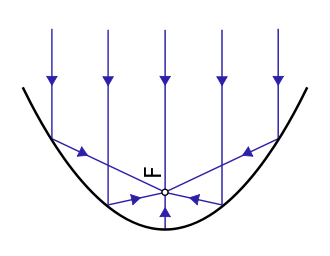
\includegraphics[scale=0.4]{parabolique.png}
	\end{center}
\end{exercice}
\begin{correction}
	A venir.
\end{correction}

\vspace*{0.5cm}
%----------------------------------------------------------------------------------------------
%-----------------------------------------------------------------------------------------------
\subsection{G\'eom\'etrie de l'espace}
\begin{exercice}
	\begin{enumerate}
		\item Déterminer l'équation du plan $P$ qui passe par les points $A ,B,C$ de coordonnées respectives :
		      $A = (1,1,1)$,  $B =(2,2,3)$ et $C =(-1,0,-2)$.
		\item Donner deux vecteurs non colinéaires et  paralléles à $P$
		\item Soit $D$ de coordonnées $(1,2,3)$.
		      Est ce que $D$ appartient à $P$ ?
		\item Donner $H$ le projeté orthogonal de $D$ sur $H$.
	\end{enumerate}
\end{exercice}
%--------------------------------------------------
\begin{correction}  \;
	\textbf{On consid\`ere les plans $\mathcal{P} : x-y+z=1$ et $\mathcal{P}' : x + 2y +3z =6$. \\
		Justifier que $\mathcal{P}\cap \mathcal{P}'$ est une droite, que l'on appellera $\cal D$. D\'eterminer un vecteur directeur de $\cal D$.}\\
	Le plan $\mathcal{P}$ admet $\vec{n}(1,-1,1)$ comme vecteur normal. Le plan $\mathcal{P}'$ admet $\vec{n'}(1,2,3)$ comme vecteur normal.\\
	$\vec{n}$ et $\vec{n'}$ ne sont pas colin\'eaires, donc $\mathcal{P}$ et $\mathcal{P}'$ ne sont pas parall\`eles. Donc leur intersection est une droite $\cal D$.\\
	Pour trouver un vecteur directeur, on cherche une \'equation param\'etrique de $\cal D$ (sachant qu'on en a une \'equation cart\'esienne).\\
	Soit $M(x,y,z)$ un point de l'espace. On r\'esout :
	$$ \left(M \in {\cal D}\right)  \iff  \begin{cases} x-y+z=1 \\ x + 2y +3z =6\end{cases}
		\underset{L_2 \leftarrow L_2-L_1}{\iff}  \begin{cases} x-y+z=1 \\ 3y +2z =5\end{cases}
		\iff  \begin{cases} x=\frac{8}{3}-\frac{5}{3}z \\ y =\frac{5}{3}-\frac{2}{3}z \\ z=z\end{cases}$$
	On obtient donc une \'equation param\'etrique de $\cal D$ : $ \begin{cases} x=\frac{8}{3}-\frac{5}{3}\lambda \\ y =\frac{5}{3}-\frac{2}{3}\lambda \\ z=0+\lambda\end{cases} \iff \begin{cases} x-\frac{8}{3}=-\frac{5}{3}\lambda \\ y -\frac{5}{3}=-\frac{2}{3}\lambda \\ z-0=\lambda\end{cases} \iff \overrightarrow{AM}=\lambda \vec{u}$,\\
	en posant $\ddp A\left(\frac{8}{3},\frac{5}{3},0\right)$ et $\ddp \vec{u}\left(-\frac{5}{3},-\frac{2}{3},1\right)$.\\
	Donc \conclusion{$\cal D$ passe par le point $\ddp A\left(\frac{8}{3},\frac{5}{3},0\right)$ et est dirig\'ee par le vecteur {$\ddp \vec{u}\left(-\frac{5}{3},-\frac{2}{3},1\right)$}.}
\end{correction}




%--------------------------------------------------
\begin{exercice}  \;
	On consid\`ere les plans $\mathcal{P} : x-y+z=1$ et $\mathcal{P}' : x + 2y +3z =6$. \\
	Justifier que $\mathcal{P}\cap \mathcal{P}'$ est une droite, que l'on appellera $\cal D$. D\'eterminer un vecteur directeur de $\cal D$.
\end{exercice}
\begin{correction}
	A venir
\end{correction}


%--------------------------------------------------


\begin{exercice}
	L'espace est rapport\'e au rep\`ere orthonorm\'e $(O,\vec{i},\vec{j},\vec{k})$. Soient les points $A(1,0,0)$, $B(0,1,0)$ et $C(0,0,2)$. Montrer que ces trois points d\'etermine un plan. Donner un vecteur normal au plan puis donner une \'equation cart\'esienne du plan.
	%L'espace est rapport\'e au rep\`ere orthonorm\'e $(O,\vec{i},\vec{j},\vec{k})$. Soient les points $A(0,1,-1)$, $B(0,0,1)$ et $C(1,-1,1)$. Montrer que ces trois points d\'eterminent un plan et en donner une \'equation cart\'esienne.
\end{exercice}

\begin{correction}
	A venir
\end{correction}




\begin{exercice}
	L'espace est rapport\'e au rep\`ere orthonorm\'e $(O,\vec{i},\vec{j},\vec{k})$. Soient $A(5,2,1)$, $\vec{u}=\vec{i}-3\vec{j}+\vec{k}$ et $\vec{v}=\vec{i}+\vec{j}$.
	\begin{enumerate}
		\item Donner une \'equation du plan passant par $A$ et de vecteurs directeurs les vecteurs $\vec{u}$ et $\vec{v}$.
		\item Donner une \'equation du plan normal \`a $\vec{u}$ et passant par $A$.
	\end{enumerate}
\end{exercice}

\begin{correction}
	A venir
\end{correction}



%--------------------------------------------------
\begin{exercice}  \;
	D\'eterminer un vecteur directeur de la  droite $\mathcal{D}$ contenant le point $A=(2,1,3)$ parall\`ele au plan d'\'equation $x+y+z=2$ et rencontrant la droite $\mathcal{D}'$ d'\'equations cart\'esiennes $x=1$ et $y=z$.
\end{exercice}


\begin{correction}  \;
	\textbf{D\'eterminer la droite $\mathcal{D}$ contenant le point $A=(2,1,3)$ parall\`ele au plan d'\'equation $x+y+z=2$ et rencontrant la droite $\mathcal{D}'$ d'\'equations cart\'esiennes $x=1$ et $y=z$.}\\
	Rassemblons les informations que l'on a :\\
	$\bullet$ ${\cal D}$ passe par le point $A=(2,1,3)$ ; il ne manque qu'un vecteur directeur de $\cal D$ pour avoir d\'etermin\'e cette droite.\\
	Appelons $\vec{u}(a,b,c)$ un vecteur directeur de $\cal D$ ($\vec{u}\neq \vec{0}$ ; on va le d\'eterminer \`a un facteur pr\`es).\\
	On aura pour \'equation param\'etrique de ${\cal D}$ :
	$$ \begin{cases} x=2+a \lambda\\ y=1+b \lambda\\ z=3+c \lambda \end{cases} ; \quad \lambda \in \R $$
	$\bullet$ ${\cal D}$ est parall\`ele au plan d'\'equation $x+y+z=2$ ; donc le vecteur $\vec{n}(1,1,1)$, qui est normal \`a ce plan, sera normal \`a $\cal D$.\\
	Donc $\vec{n}.\vec{u}=0$. Donc $a+b+c=0$, donc \conclusion{$a=-b-c$}. D'o\`u l'\'equation param\'etrique de $\cal D$ :
	$$ \begin{cases} x=2+(-b-c) \lambda\\ y=1+b \lambda\\ z=3+c \lambda \end{cases} ; \quad \lambda\in \R $$
	$\bullet$ ${\cal D}$ rencontre la droite $\mathcal{D}'$ d'\'equations cart\'esiennes $x=1$ et $y=z$.\\
	Donc le syst\`eme suivant, d'inconnue $\lambda$, admet au moins une solution.
	$$ (S) : \begin{cases} 2+(-b-c) \lambda=1\\ 1+b \lambda=3+c \lambda \end{cases} \iff \begin{cases} (b+c) \lambda=1\\ (b-c) \lambda=2 \end{cases} $$
	On doit donc avoir \conclusion{$b+c \neq 0$} (sinon la premi\`ere \'equation n'a pas de solution), et on obtient :
	$$ (S) \iff \begin{cases} \lambda=\frac{1}{b+c}\\ \frac{b-c}{b+c}=2 \end{cases} \iff \begin{cases} \lambda=\frac{1}{b+c}\\ b-c=2b+2c \end{cases} \iff \begin{cases} \lambda=\frac{1}{b+c}\\ b=-3c \end{cases}  $$
	Rassemblons les informations sur les coordonn\'ees du vecteur $\text{u}(a,b,c)$ :
	$$ \begin{cases} a = -b-c \\ b+c \neq 0 \\ b=-3c \end{cases} \iff \begin{cases} a=2c \\ b=-3c \\ c \neq 0\end{cases}$$
	On a un param\`etre libre : c'est normal, une infinit\'e de vecteurs conviennent ; on peut par exemple poser $c=1$, et l'on obtient $a=2$ et $b=-3$.\\
	Donc \conclusion{$\vec{u}(2,-3,1)$}.\\
	\conclusion{$\cal D$ est la droite passant par $A=(2,1,3)$ et dirig\'ee par $\vec{u}(2,-3,1)$}. Elle a pour \'equation param\'etrique :
	$$ \begin{cases} x=2+2 \lambda\\ y=1-3 \lambda\\ z=3+ \lambda \end{cases} ; \quad \lambda\in \R $$
\end{correction}



%--------------------------------------------------
%\begin{exercice}  \;
%D\'eterminer l'\'equation de la sph\`ere $\mathcal{S}$ dans chacun des cas suivants :
%\begin{enumerate}
%\item $\mathcal{S}$ est de centre $\Omega(-1,2,4)$ et passe par $A(1,2,-1)$.
%\item $\mathcal{S}$ est de diam\`etre $[AB]$ o\`u $A(1,2,5)$ et $B(3,-4,1)$.
%\item $\mathcal{S}$ est de centre $\Omega(3,-4,2)$ et est tangente au plan d'\'equation $2x-6y+3z-8=0$.
%\end{enumerate}
%\end{exercice}
%--------------------------------------------------
%\begin{correction}  \;
%\textbf{D\'eterminer l'\'equation de la sph\`ere $\mathcal{S}$ dans chacun des cas suivants :}
%\begin{enumerate}
%%---
%\item \textbf{$\mathcal{S}$ est de centre $\Omega(-1,2,4)$ et passe par $A(1,2,-1)$.}\\
%Il suffit de trouver le rayon de la sph\`ere, et pour cela de calculer la distance $\Omega A$. On a $\Omega A = \sqrt{(1+1)^2+(2-2)^2+(-1-4)^2} = \sqrt{29}$. \\
%On applique ensuite la formule du cours et on obtient : \conclusion{$\mathcal{S} : (x+1)^2+(y-2)^2+(z-4)^2 = 29$}.
%%---
%\item \textbf{$\mathcal{S}$ est de diam\`etre $[AB]$ o\`u $A(1,2,5)$ et $B(3,-4,1)$.}\\
%On commence par calculer le rayon. On a $AB = \sqrt{(3-1)^2+(-4-2)^2+(1-5)^2} = \sqrt{56} = 2 \sqrt{14}$. Donc le rayon de la sp\`ere est $\ddp \frac{AB}{2} = \sqrt{14}$. Il reste \`a trouver les coordonn\'ees du centre. Pour cela on cherche le milieu de $AB$, qui a pour coordonn\'ees $\ddp \Omega = \left( \frac{1+3}{2}, \frac{2-4}{2}, \frac{5+1}{2}\right) = (2,-1,3)$. On applique ensuite la formule du cours et on obtient : \conclusion{$\mathcal{S} : (x-2)^2+(y+1)^2+(z-3)^2 = 14$}.
%%---
%\item \textbf{$\mathcal{S}$ est de centre $\Omega(3,-4,2)$ et est tangente au plan d'\'equation $2x-6y+3z-8=0$.}\\
%Notons $A(x,y,z)$ l'unique point d'intersection entre la sp\`ere et le plan. On sait que $\overrightarrow{\Omega A}$ est un vecteur normal au plan. Or, tous les vecteurs normaux au plan sont colin\'eaires au vecteur $(2,-6,3)$, donc il existe $\lambda \in \R$ tel que $\overrightarrow{\Omega A} = \lambda (2,-6,3)$. On en d\'eduit que l'on a :
%$$\left\{ \begin{array}{rcl}
%x-3 & = & 2\lambda\vsec\\
%y+4 & = & -6 \lambda \vsec\\
%z-2 & = & 3 \lambda
%\end{array}\right.
%\Leftrightarrow 
%\left\{ \begin{array}{rcl}
%x& = & 3+2\lambda\vsec\\
%y & = & -4-6 \lambda \vsec\\
%z & = & 2+3 \lambda
%\end{array}\right.$$ 
%De plus, comme $A$ appartient au plan, ses coordonn\'ees v\'erifie l'\'equation :
%$$2x-6y+3z-8=0 \Leftrightarrow  2(3+2\lambda) - 6 (-4-6 \lambda) + 3(2+3 \lambda) -8 = 0 \Leftrightarrow \lambda = -\frac{4}{7}.$$
%On en d\'eduit que le rayon de la sph\`ere est donn\'e par 
%$$\Omega A = \left|\left|-\frac{4}{7} (2,-6,3) \right|\right| = \frac{4}{7} \sqrt{2^2+(-6)^2+3^2} = 28.$$
% On applique ensuite la formule du cours et on obtient : \conclusion{$\mathcal{S} : (x-3)^2+(y+4)^2+(z-2)^2 = 28^2$}.
%\end{enumerate}
%\end{correction}






\subsection*{Produit scalaire}

\begin{exercice}  \;
	Soient $\vec{u}$ et $\vec{v}$ deux vecteurs du plan.
	\begin{enumerate}
		\item D\'emontrer que $\vec{u}$ et $\vec{v}$ sont orthogonaux si et seulement si $\| \vec{u}+ \vec{v}\| = \| \vec{u}-\vec{v}\|$.
		\item D\'eduire de la question pr\'ec\'edente, une condition n\'ecessaire et suffisante pour qu'un parall\'elogramme $ABCD$ soit rectangle.
	\end{enumerate}
\end{exercice}
\begin{correction}  \;
	\textbf{Soient $\vec{u}$ et $\vec{v}$ deux vecteurs du plan.}
	\begin{enumerate}
		\item \textbf{D\'emontrer que $\vec{u}$ et $\vec{v}$ sont orthogonaux si et seulement si $\| \vec{u}+ \vec{v}\| = \| \vec{u}-\vec{v}\|$.}\\
		      On calcule :
		      $$\| \vec{u}+ \vec{v}\|^2 = \| \vec{u}\|^2 + \| \vec{v}\|^2 + 2 \vec{u} \cdot \vec{v}$$
		      $$\| \vec{u}- \vec{v}\|^2 = \| \vec{u}\|^2 + \| \vec{v}\|^2 - 2 \vec{u} \cdot \vec{v}$$
		      Donc :
		      $$\| \vec{u}+ \vec{v}\|^2 - \| \vec{u}- \vec{v}\|^2 = 4 \vec{u} \cdot \vec{v}$$
		      Comme $\| \vec{u}+ \vec{v}\| \in \R_+$, $\| \vec{u}- \vec{v}\| \in \R_+$ et $x \mapsto x^2$ est strictement croissante sur $\R_+$, on r\'esout :
		      $$ \left(\| \vec{u}+ \vec{v}\| = \| \vec{u}- \vec{v}\|\right) \iff \left(\| \vec{u}+ \vec{v}\|^2 = \| \vec{u}- \vec{v}\|^2\right) \iff \left(\| \vec{u}+ \vec{v}\|^2 - \| \vec{u}- \vec{v}\|^2 = 0\right) \iff \left( 4 \vec{u} \cdot \vec{v} = 0\right)$$
		      $$ \iff \left( \vec{u} \cdot \vec{v} = 0\right) \iff \left(\vec{u}\text{ et }\vec{v}\text{ sont orthogonaux}\right)$$
		      Conclusion : \conclusion{$\vec{u}$ et $\vec{v}$ sont orthogonaux si et seulement si $\| \vec{u}+ \vec{v}\| = \| \vec{u}-\vec{v}\|$.}
		      %------
		\item \textbf{D\'eduire de la question pr\'ec\'edente, une condition n\'ecessaire et suffisante pour qu'un parall\'elogramme $ABCD$ soit rectangle.}\\
		      Faites un dessin pour voir de quoi vous parlez !\\
		      Soit $ABCD$ un parall\'elogramme. On r\'esout :
		      $$  \left(ABCD\text{ est un rectangle}\right) \iff \left( \overrightarrow{AB} \text{ et }\overrightarrow{AD} \text{ sont orthogonaux}\right) \iff \left( \left\| \overrightarrow{AB} +\overrightarrow{AD} \right\| = \left\| \overrightarrow{AB} -\overrightarrow{AD} \right\| \right)$$
		      $$ \iff \left( \left\| \overrightarrow{AB} +\overrightarrow{BC} \right\| = \left\| \overrightarrow{AB} +\overrightarrow{DA} \right\| \right) \iff \left( \left\| \overrightarrow{AC} \right\| = \left\| \overrightarrow{DB} \right\| \right) \iff \left(AC=DB\right) $$
		      Conclusion : \conclusion{$ABCD$ est un rectangle, si et seulement si ses diagonales sont de m\^eme longueur.}
	\end{enumerate}
\end{correction}
%--------------------------------------------------
%--------------------------------------------------
\begin{exercice}  \;
	Soit $ABC$ un triangle non plat du plan.
	\begin{enumerate}
		\item D\'emontrer que, pour tout point $M$ du plan, on a $\overrightarrow{MA}.\overrightarrow{BC} + \overrightarrow{MB}.\overrightarrow{CA} + \overrightarrow{MC}.\overrightarrow{AB} = 0$.
		\item Soit $H$ le point d'intersection des hauteurs issues de $B$ et $C$. \\
		      Montrer que $\overrightarrow{HA}.\overrightarrow{BC} = 0$ et en d\'eduire que $H$ appartient \`a la hauteur issue de $A$.
	\end{enumerate}
\end{exercice}
\begin{correction}  \;
	\textbf{Soit $ABC$ un triangle non plat du plan.}
	\begin{enumerate}
		\item \textbf{D\'emontrer que, pour tout point $M$ du plan, on a $\mathbf{\overrightarrow{MA}.\overrightarrow{BC} + \overrightarrow{MB}.\overrightarrow{CA} + \overrightarrow{MC}.\overrightarrow{AB} = 0}$.}\\
		      Soit $M$ un point du plan. On calcule :\\
		      $$\begin{array}{lcl}\overrightarrow{MA}.\overrightarrow{BC} + \overrightarrow{MB}.\overrightarrow{CA} + \overrightarrow{MC}.\overrightarrow{AB} & = & \overrightarrow{MA}.\overrightarrow{BC} + \left(\overrightarrow{MA}+\overrightarrow{AB}\right).\overrightarrow{CA} + \left(\overrightarrow{MA}+\overrightarrow{AC}\right).\overrightarrow{AB} \\
                                                                                                                                              & = & \overrightarrow{MA}.\left(\overrightarrow{BC} + \overrightarrow{CA} +\overrightarrow{AB}\right) + \overrightarrow{AB}.\overrightarrow{CA} +\overrightarrow{AC}.\overrightarrow{AB}            \\
                                                                                                                                              & = & \overrightarrow{MA}.\left(\overrightarrow{BB}\right) + \left(\overrightarrow{CA} +\overrightarrow{AC}\right).\overrightarrow{AB}                                                              \\
                                                                                                                                              & = & 0+0                                                                                                                                                                                           \\
                                                                                                                                              & = & 0\end{array}$$
		      %------
		\item \textbf{Soit $H$ le point d'intersection des hauteurs issues de $B$ et $C$. \\
			      Montrer que $\mathbf{\overrightarrow{HA}.\overrightarrow{BC} = 0}$ et en d\'eduire que $H$ appartient \`a la hauteur issue de $A$.}\\
		      Soit $H$ le point d'intersection des hauteurs issues de $B$ et $C$. \\
		      $\bullet$ $H$ appartient \`a la hauteur issue de $B$ donc les droites $(HB)$ et $(CA)$ sont perpendiculaires, donc :$$\overrightarrow{HB}.\overrightarrow{CA} = 0$$
		      $\bullet$ $H$ appartient \`a la hauteur issue de $C$ donc les droites $(HC)$ et $(AB)$ sont perpendiculaires, donc :$$\overrightarrow{HC}.\overrightarrow{AB} = 0$$
		      On en d\'eduit, en appliquant {\bf 1} :
		      $\overrightarrow{HA}.\overrightarrow{BC} + \overrightarrow{HB}.\overrightarrow{CA} + \overrightarrow{HC}.\overrightarrow{AB}=0$, donc $\overrightarrow{HA}.\overrightarrow{BC} + 0+0=0$, donc $\overrightarrow{HA}.\overrightarrow{BC} = 0$, donc les droites $(HA)$ et $(BC)$ sont perpendiculaires, donc $H$ appartient \`a la hauteur issue de $A$.
	\end{enumerate}
\end{correction}
%--------------------------------------------------
%--------------------------------------------------
\begin{exercice}  \; Formule d'Al Kachi.\\
	On consid\`ere un triangle $ABC$. On note $\hat{A}$, $\hat{B}$ et $\hat{C}$ les mesures respectives des angles non orient\'es $\widehat{BAC}$, $\widehat{ABC}$ et $\widehat{ACB}$ et l'on pose $a=BC$, $b=AC$ et $c=AB$.
	\begin{enumerate}
		\item D\'emontrer que $a^2=b^2+c^2-2bc\cos(\hat{A})$ et \'enoncer deux autres formules similaires. Qu'obtient-on si $\hat{A} = \ddp\frac{\pi}{2}$?
		\item Si $a=4$, $b=3$ et $c=2$, calculer une valeur approch\'ee (\`a $10^{-2}$ degr\'e pr\`es) de $\hat{A}$, $\hat{B}$ et $\hat{C}$.
		\item Si $\hat{A} = \ddp\frac{\pi}{6}$, $a=3$ et $c=2$, calculer $b$.
	\end{enumerate}
\end{exercice}
\begin{correction}  \; Formule d'Al Kachi.\\
	\textbf{On consid\`ere un triangle $ABC$. On note $\hat{A}$, $\hat{B}$ et $\hat{C}$ les mesures respectives des angles non orient\'es $\widehat{BAC}$, $\widehat{ABC}$ et $\widehat{ACB}$ et l'on pose $a=BC$, $b=AC$ et $c=AB$.}
	\begin{enumerate}
		\item \textbf{D\'emontrer que $a^2=b^2+c^2-2bc\cos(\hat{A})$ et \'enoncer deux autres formules similaires. Qu'obtient-on si $\hat{A} = \frac{\pi}{2}$?}\\
		      On calcule :
		      $$ a^2=BC^2=\left\|\overrightarrow{BC}\right\|^2 = \left\|\overrightarrow{BA}+\overrightarrow{AC}\right\|^2 = \left\|\overrightarrow{BA}\right\|^2+\left\|\overrightarrow{AC}\right\|^2+2 \overrightarrow{BA}.\overrightarrow{AC} = c^2+b^2-2 \overrightarrow{AB}.\overrightarrow{AC} = c^2+b^2-2bc\cos(\hat{A})$$
		      De m\^eme : $b^2=c^2+a^2-2ac\cos(\hat{B})$ et  $c^2=a^2+b^2-2ab\cos(\hat{C})$.\\
		      Si $\hat{A} = \frac{\pi}{2}$, donc si le triangle $ABC$ est rectangle en $A$, on obtient $\cos(\hat{A})=0$, donc :\\$a^2=b^2+c^2$ : c'est le th\'eor\`eme de Pythagore.
		      %-----
		\item \textbf{Si $a=4$, $b=3$ et $c=2$, calculer une valeur approch\'ee (\`a $10^{-2}$ degr\'e pr\`es) de $\hat{A}$, $\hat{B}$ et $\hat{C}$.}\\
		      $\cos(\hat{A})=\ddp\frac{-a^2+b^2+c^2}{2bc}=-\frac{1}{4}$, et $\hat{A} \in [0;\pi]$ (angle non orient\'e), donc $\ddp\hat{A} = \arccos\left(-\frac{1}{4}\right) \approx 104,48^{\circ}$.\\
		      $\cos(\hat{B})=\ddp\frac{-b^2+a^2+c^2}{2ac}=\frac{11}{16}$, et $\hat{B} \in [0;\pi]$ (angle non orient\'e), donc $\ddp\hat{B} = \arccos\left(\frac{11}{16}\right) \approx 46,57^{\circ}$.\\
		      $\cos(\hat{C})=\ddp\frac{-c^2+a^2+b^2}{2ab}=\frac{21}{24}$, et $\hat{C} \in [0;\pi]$ (angle non orient\'e), donc $\ddp\hat{C} = \arccos\left(\frac{21}{24}\right) \approx 28.96^{\circ}$.\\
		      Remarque : on peut v\'erifier que $\hat{A}+\hat{B}+\hat{C}\approx 180^{\circ}$ (\`a $0,01^{\circ}$ pr\`es).\\
		      %-----
		\item \textbf{Si $\hat{A} = \frac{\pi}{6}$, $a=3$ et $c=2$, calculer $b$.}\\
		      $\ddp a^2=c^2+b^2-2bc\cos(\hat{A})$, donc $b^2-2bc\cos(\hat{A})+c^2-a^2=0$, donc $b^2-2\sqrt{3}\, b-5=0$.\\
		      Le discriminant de cette \'equation vaut $\Delta=32=\left(4\sqrt{2}\right)^2$, donc :\\
		      $b=\ddp\frac{2\sqrt{3}+4\sqrt{2}}{2}=\sqrt{3}+2\sqrt{2}$ ou $b=\ddp\frac{2\sqrt{3}-4\sqrt{2}}{2}=\sqrt{3}-2\sqrt{2}$.\\
		      Or $b \geq 0$ (c'est une longueur), donc \conclusion{$b=\sqrt{3}-2\sqrt{2}$}.
	\end{enumerate}
\end{correction}

\vspace{0.5cm}

%------------------------------------------------
%----------------------------------------------------------------------------------------------
%-----------------------------------------------------------------------------------------------
\subsection*{G\'eom\'etrie et nombres complexes}

%--------------------------------------------------
%--------------------------------------------------
\begin{exercice}  \;
	D\'eterminer g\'eom\'etriquement les complexes $z$ v\'erifiant les relations suivantes. V\'erifier votre r\'esultat par un calcul.
	\begin{enumerate}
		\item $|z-1-i| = |z+1+i|$
		\item $(|z-i|-1)(|z+1|-2)=0$
		\item $\ddp\frac{z-1}{z-i} \in \R_+^{\star}$
	\end{enumerate}
\end{exercice}
\begin{correction}  \;
	\textbf{D\'eterminer g\'eom\'etriquement les complexes $z$ v\'erifiant les relations suivantes. V\'erifier votre r\'esultat par un calcul.}
	\begin{enumerate}
		\item $\mathbf{|z-1-i| = |z+1+i|}$:\\
		      %\begin{minipage}[c]{0.5\linewidth}
		      Soit $A$, $B$ et $M$ les points d'affixes $1+i$, $-1-i$ et $z$. On a :
		      $$|z-1-i| = |z+1+i| \Leftrightarrow AM=BM,$$
		      donc l'ensemble des points cherch\'es est \conclusion{la m\'ediatrice du segment $[AB]$.}
		      %\end{minipage} 
		      \hspace*{0.5cm}
		      %\begin{minipage}[c]{0.4\linewidth}
		      %%\begin{center}
		      %%\includegraphics[width=0.9\linewidth]{./Figures/complexes1.eps}
		      %%\end{center}
		      %\end{minipage}\\
		      \noindent On retrouve ce r\'esultat par le calcul. Soit $(x,y)\in \R^2$ tels que $z=x+iy$. On a alors :
		      $$\hspace*{-1cm}\begin{array}{rcll}
				      |z-1-i| = |z+1+i| & \Leftrightarrow & |x+iy-1-i| = |x+iy+1+i|\vsec                                                                         \\
				                        & \Leftrightarrow & \sqrt{(x-1)^2+(y-1)^2} =  \sqrt{(x+1)^2+(y+1)^2}\vsec                                                \\
				                        & \Leftrightarrow & (x-1)^2+(y-1)^2 = (x+1)^2+(y+1)^2                     & \textmd{ car les termes sont positifs }\vsec \\
				                        & \Leftrightarrow & x^2-2x+1+y^2-2y+1 = x^2+2x +1 +y^2+2y+1\vsec                                                         \\
				                        & \Leftrightarrow & y =-x
			      \end{array}$$
		      Ainsi l'ensemble solution est \conclusion{la droite d'\'equation $y=-x$}.
		      %----
		\item $\mathbf{(|z-i|-1)(|z+1|-2)=0}$:\\
		      %\begin{minipage}[c]{0.5\linewidth}
		      Soit $A$, $B$ et $M$ les points d'affixes $i$, $-1$ et $z$. On a :
		      $$\begin{array}{rcl}
				      (|z-i|-1)(|z+1|-2)=0 & \Leftrightarrow & |z-i|-1=0 \textmd{ ou } |z+1|-2=0\vsec \\
				                           & \Leftrightarrow & AM= 1  \textmd{ ou }  BM=2
			      \end{array},$$
		      donc l'ensemble des points cherch\'es est \conclusion{la r\'eunion des cercles $\mathcal{C}(A,1)$ et $\mathcal{C}(B,2)$.}
		      %\end{minipage} 
		      \hspace*{0.5cm}
		      %\begin{minipage}[c]{0.4\linewidth}
		      %\begin{center}
		      %\includegraphics[width=0.9\linewidth]{./Figures/complexes2.eps}
		      %\end{center}
		      %\end{minipage}\\
		      \noindent On retrouve ce r\'esultat par le calcul. Soit $(x,y)\in \R^2$ tels que $z=x+iy$. On a alors :
		      $$\hspace*{-1cm}\begin{array}{rcll}
				      |z-i|-1=0 \textmd{ ou } |z+1|-2=0 & \Leftrightarrow & |x+iy-i|=1 \textmd{ ou } |x+iy+1|=2\vsec                                                                     \\
				                                        & \Leftrightarrow & \sqrt{x^2+(y-1)^2} = 1 \textmd{ ou }   \sqrt{(x+1)^2+y^2} = 2\vsec                                           \\
				                                        & \Leftrightarrow & x^2+(y-1)^2 =1 \textmd{ ou }   (x+1)^2+y^2 =  4                    & \textmd{ car les termes sont positifs }\end{array}$$
		      Ainsi l'ensemble solution est bien la r\'eunion des deux cercles trouv\'es pr\'ec\'edemment.
		      %----
		\item $\mathbf{\ddp\frac{z-1}{z-i} \in \R_+^{\star}}$:Soit $A$, $B$ et $M$ les points d'affixes $i$, $1$ et $z$. On a :\\
		      %\begin{minipage}[c]{0.5\linewidth}
		      $$\ddp\frac{z-1}{z-i} \in \R_+^{\star}  \Leftrightarrow \exists \lambda \in \R_+^{\star}, \frac{z-1}{z-i} = \lambda$$
		      $$\begin{array}{rcl}
				      \ddp\frac{z-1}{z-i} \in \R_+^{\star} & \Leftrightarrow & \exists \lambda \in \R_+^{\star}, \ddp \frac{z-1}{z-i} = \lambda\vsec               \\
				                                           & \Leftrightarrow & \exists \lambda \in \R_+^{\star}, z-1 = \lambda(z-i) \vsec                          \\
				                                           & \Leftrightarrow & \exists \lambda \in \R_+^{\star}, \overrightarrow{AM} = \lambda \overrightarrow{BM}
			      \end{array},$$
		      donc l'ensemble des points cherch\'es est l'ensemble des points de la droite $(AB)$ pour lesquels les vecteurs $\overrightarrow{AM}$ et $\overrightarrow{BM}$ sont colin\'eaires de m\^eme sens (car $\lambda >0$). On obtient  \conclusion{la r\'eunion de deux demi-droites.}
		      %\end{minipage} 
		      \hspace*{0.5cm}
		      %\begin{minipage}[c]{0.4\linewidth}
		      %\begin{center}
		      %\includegraphics[width=0.9\linewidth]{./Figures/complexes3.eps}
		      %\end{center}
		      %\end{minipage}\\
		      \noindent On retrouve ce r\'esultat par le calcul. Soit $(x,y)\in \R^2$ tels que $z=x+iy$. Soit $\lambda \in \R_+^\star$ tel que
		      $$\hspace*{-1cm}\begin{array}{rcll}
				      z-1 = \lambda(z-i) & \Leftrightarrow & x+iy-1 = \lambda(x+iy-i)\vsec                                                               \\
				                         & \Leftrightarrow & \left\{\begin{array}{rcl}
					                                                    x-1 & = & \lambda x\vsec \\
					                                                    y   & = & \lambda (y-1)
				                                                    \end{array}\right.\vsec                                                             \\
				                         &                 & \textmd{ par identification des parties r\'eelles et imaginaires}\vsec                      \\
				                         & \Leftrightarrow & \left\{\begin{array}{rcll}
					                                                    \lambda & = & \ddp \frac{x-1}{x}       & \textmd{ car $x=0$ n'est pas solution}\vsec \\
					                                                    y       & = & \ddp \frac{x-1}{x} (y-1)
				                                                    \end{array}\right.
			      \end{array}$$
		      La derni\`ere \'equation donne : $xy  =  \ddp (x-1)(y-1) \Leftrightarrow xy = xy-x-y+1 \Leftrightarrow y=-x+1$. De plus, on a : $\lambda >0 \Leftrightarrow \ddp \frac{x-1}{x} >0 \Leftrightarrow x \in ]-\infty,0[ \; \cup \; ]1, +\infty[$.
		      Ainsi l'ensemble solution est bien la r\'eunion des deux demi-droites trouv\'ees pr\'ec\'edemment.
	\end{enumerate}
\end{correction}
%--------------------------------------------------
%--------------------------------------------------

\vspace{0.5cm}

%------------------------------------------------
%----------------------------------------------------------------------------------------------
%-----------------------------------------------------------------------------------------------
%\noindent \section{{\bf\Large{Barycentres}}}
%
%%\begin{exercice}
%%On donne les points $A=(-1,3)$, $B=(2,-1)$ et $C=(3,4)$. \\
%%D\'eterminer les coordonn\'ees du barycentre $G$ du syst\`eme $\{(A,-1),(B,2),(C,3)\}$.
%%\end{exercice}
%\begin{correction}
%\textbf{On donne les points $A=(-1,3)$, $B=(2,-1)$ et $C=(3,4)$. \\
%D\'eterminer les coordonn\'ees du barycentre $G$ du syst\`eme $\{(A,-1),(B,2),(C,3)\}$.}\\
%Le barycentre $G(x_G,y_G)$ v\'erifie par d\'efinition :\\
%$\bullet$ $x_G = \ddp \frac{1}{-1+2+3}\left(-x_A+2x_B+3x_C\right) = \frac{1}{4}\left(-(-1)+2\times 2+3 \times 3\right) = \frac{7}{2}$.\\
%$\bullet$ $y_G = \ddp \frac{1}{-1+2+3}\left(-y_A+2y_B+3y_C\right) = \frac{1}{4}\left(-3+2\times (-1)+3 \times 4\right) = \frac{7}{4}$.\\
%Donc \conclusion{$\ddp G\left(\frac{7}{2},\frac{7}{4}\right)$}.\\
%\end{correction}
%%--------------------------------------------------
%%--------------------------------------------------
%\begin{exercice}  \;
%Soient $A$, $B$, $C$, $A'$, $B'$ et $C'$ six points du plan. On note $G$ et $G'$ les isobarycentres respectifs des familles $(A,B,C)$ et $(A',B',C')$.
%\begin{enumerate}
% \item Montrer que $\overrightarrow{AA'}+\overrightarrow{BB'}+\overrightarrow{CC'}=3\overrightarrow{GG'}$
%\item Montrer que $G$ et $G'$ sont confondus, si et seulement s'il existe un point $M$ tel que les quadrilat\`eres $BA'CM$ et $B'AC'M$ soient des parall\'elogrammes.
%\end{enumerate}
%\end{exercice}
%\begin{correction}  \;
%\textbf{Soient $A$, $B$, $C$, $A'$, $B'$ et $C'$ six points du plan. On note $G$ et $G'$ les isobarycentres respectifs des familles $(A,B,C)$ et $(A',B',C')$.}
%\begin{enumerate}
%\item \textbf{Montrer que $\overrightarrow{AA'}+\overrightarrow{BB'}+\overrightarrow{CC'}=3\overrightarrow{GG'}$}\\
%$G$ est l'isobarycentre de $(A,B,C)$, donc $\overrightarrow{GA}+\overrightarrow{GB}+\overrightarrow{GC}=\vec{0}$, et donc $\overrightarrow{AG}+\overrightarrow{BG}+\overrightarrow{CG}=\vec{0}$.\\
%$G'$ est l'isobarycentre de $(A',B',C')$, donc $\overrightarrow{G'A'}+\overrightarrow{G'B'}+\overrightarrow{G'C'}=\vec{0}$.\\
%On use et on abuse de la relation de Chasles, en introduisant $G$ et $G'$ puisqu'on les veut dans le membre de gauche. On calcule :
%$$ \begin{array}{lcl} \overrightarrow{AA'}+\overrightarrow{BB'}+\overrightarrow{CC'} & = & \left(\overrightarrow{AG}+\overrightarrow{GG'}+\overrightarrow{G'A'}\right)+\left(\overrightarrow{BG}+\overrightarrow{GG'}+\overrightarrow{G'B'}\right)+\left(\overrightarrow{CG}+\overrightarrow{GG'}+\overrightarrow{G'C'}\right) \\
%& = & \left(\overrightarrow{AG}+\overrightarrow{BG}+\overrightarrow{CG}\right)+\left(\overrightarrow{G'A'}+\overrightarrow{G'B'}+\overrightarrow{G'C'}\right)+3\overrightarrow{GG'} \\
%& = & 3\overrightarrow{GG'} \end{array} $$
%%----
%\item \textbf{Montrer que $G$ et $G'$ sont confondus, si et seulement s'il existe un point $M$ tel que les quadrilat\`eres $BA'CM$ et $B'AC'M$ soient des parall\'elogrammes.}\\
%Rappel : pour un point $M$ donn\'e, on a l'\'equivalence :\\
%($BA'CM$ et $B'AC'M$ sont des parall\'elogrammes) $\iff$ ($\overrightarrow{BA'}=\overrightarrow{MC}$ et $\overrightarrow{B'A}=\overrightarrow{MC'}$)\\
%
%On en d\'eduit les \'equivalences suivantes (on utilise la relation de Chasles pour faire dispara\^itre $M$) :\\
%(il existe un point $M$ tel que $BA'CM$ et $B'AC'M$ soient des parall\'elogrammes) \\
%$\iff$ (il existe un point $M$ tel que $\overrightarrow{BA'}=\overrightarrow{MC}$ et $\overrightarrow{B'A}=\overrightarrow{MC'}$)\\
%$\iff$ (il existe un point $M$ tel que $\overrightarrow{BA'}=\overrightarrow{MC}$ et $\overrightarrow{BA'}-\overrightarrow{B'A}=\overrightarrow{MC}-\overrightarrow{MC'}$)\\
%$\iff$ (il existe un point $M$ tel que $\overrightarrow{BA'}=\overrightarrow{MC}$ et $\overrightarrow{BA'}-\overrightarrow{B'A}=\overrightarrow{C'C}$)\\
%$\iff$ ($\overrightarrow{BA'}-\overrightarrow{B'A}=\overrightarrow{C'C}$)\\
%(en effet, il existera toujours un point $M$ tel que $\overrightarrow{BA'}=\overrightarrow{MC}$)\\
%
%Calculons donc $\overrightarrow{BA'}$ en utilisant la question {\bf 1} :
%$$ \overrightarrow{BA'} = \overrightarrow{BA} + \overrightarrow{AA'} = \overrightarrow{BA} + 3\overrightarrow{GG'} - \overrightarrow{BB'} - \overrightarrow{CC'} = \overrightarrow{B'A} + 3\overrightarrow{GG'} - \overrightarrow{CC'} $$
%Donc :
%$$ \overrightarrow{BA'} - \overrightarrow{B'A} = 3\overrightarrow{GG'} + \overrightarrow{C'C} $$
%
%On peut \`a pr\'esent raisonner par \'equivalences :
%$$ \begin{array}{lcl} \left(G \text{ et } G' \text{ sont confondus}\right) & \iff & \overrightarrow{GG'}=\vec{0} \\
%& \iff & 3\overrightarrow{GG'}+\overrightarrow{C'C}=\overrightarrow{C'C} \\
%& \iff & \overrightarrow{BA'} - \overrightarrow{B'A} = \overrightarrow{C'C} \\ 
%& \iff & (\text{il existe } M \text{ tel que } BA'CM \text{ et } B'AC'M \text{ soient des parall\'elogrammes}) \end{array}$$
%\end{enumerate}
%\end{correction}
%%--------------------------------------------------
%%--------------------------------------------------
%\begin{exercice}  \;
%Soit $ABCD$ un t\'etra\`edre de l'espace. D\'eterminer, en fonction de $k\in \R$, l'ensemble $\mathcal{S}_k$ des points $M$ de l'espace tels que $\left(\overrightarrow{MA}+\overrightarrow{MB} + \overrightarrow{MC}\right) \cdot \overrightarrow{MD} = 3k$. \textit{On pourra introduire le barycentre} $G$ \textit{de} $(A,1),(B,1),(C,1)$ \textit{et} $(D,3)$.
%\end{exercice}
%
%\begin{correction}  \;
%\textbf{Soit $ABCD$ un t\'etra\`edre de l'espace. D\'eterminer, en fonction de $k\in \R$, l'ensemble $\mathcal{S}_k$ des points $M$ de l'espace tels que $\left(\overrightarrow{MA}+\overrightarrow{MB} + \overrightarrow{MC}\right) \cdot \overrightarrow{MD} = 3k$. \textit{On pourra introduire le barycentre} $G$ \textit{de} $(A,1),(B,1),(C,1)$\textit{et} $(D,3)$.}\\
%Posons $G$ le barycentre $(A,1),(B,1),(C,1)$ et $(D,3)$.
%Alors $\overrightarrow{GA}+\overrightarrow{GB} + \overrightarrow{GC} + 3 \overrightarrow{GD} = \vec{0}$.\\
%Soit $M$ un point de l'espace. %Alors $\overrightarrow{MA}+\overrightarrow{MB} + \overrightarrow{MC} + 3 \overrightarrow{MD} = 6 \overrightarrow{MG}$.\\
%On r\'esout, en introduisant $G$ avec la relation de Chasles :
%$$ \begin{array}{ccc} \left(\overrightarrow{MA}+\overrightarrow{MB} + \overrightarrow{MC}\right) \cdot \overrightarrow{MD} = 3k & \iff &  \left(\overrightarrow{MG}+\overrightarrow{GA}+\overrightarrow{MG}+\overrightarrow{GB} + \overrightarrow{MG}+\overrightarrow{GC}\right) \cdot \left(\overrightarrow{MG}+\overrightarrow{GD}\right) = 3k \\
%& \iff & \left(3 \overrightarrow{MG}-3 \overrightarrow{GD}\right) \cdot \left(\overrightarrow{MG}+\overrightarrow{GD}\right) = 3k \\
%& \iff & \left(\overrightarrow{MG}- \overrightarrow{GD}\right) \cdot \left(\overrightarrow{MG}+\overrightarrow{GD}\right) = k \\
%& \iff & \left\|\overrightarrow{MG}\right\|^2 - \left\|\overrightarrow{GD}\right\|^2 = k \\
% & \iff & MG^2 = GD^2 + k  \end{array}$$
%\begin{enumerate}
%\item Premier cas : $k<-GD^2$. Alors $GD^2 + k<0$ et il n'y a pas de solution.
%\item Deuxi\`eme cas : $k=-GD^2$. Alors $\left(\overrightarrow{MA}+\overrightarrow{MB} + \overrightarrow{MC}\right) \cdot \overrightarrow{MD} = 3k \iff MG=0 \iff M=G$.
%L'ensemble des solutions est r\'eduit au point $G$.
%\item Troisi\`eme cas : $k>-GD^2$. Alors $\left(\overrightarrow{MA}+\overrightarrow{MB} + \overrightarrow{MC}\right) \cdot \overrightarrow{MD} = 3k \iff MG=\sqrt{GD^2 + k} $.\\
%L'ensemble des solutions est le cercle de centre $G$ et de rayon $\sqrt{GD^2 + k }$.
%\end{enumerate}
%\end{correction}
%
%
%%\vspace{1cm}
%\newpage

%------------------------------------------------
%----------------------------------------------------------------------------------------------
%-----------------------------------------------------------------------------------------------

\end{document}